\documentclass{article}
\PassOptionsToPackage{numbers,sort&compress}{natbib}
\makeatletter
\def\input@path{{template/}}
\makeatother
\usepackage[dblblindworkshop]{neurips_2026}
\workshoptitle{AI for Drug Discovery: Bridging the Translation Gap}
\makeatletter
\renewcommand{\@noticestring}{Submitted to the AI for Drug Discovery workshop (NeurIPS 2026).}
\makeatother
\usepackage{amsmath}
\usepackage{amssymb}
\usepackage{amsthm}
\usepackage{booktabs}
\usepackage{graphicx}
\usepackage{microtype}
\usepackage{xcolor}
\usepackage{url}
\usepackage{hyperref}
\hypersetup{hidelinks}
\usepackage{enumitem}
\setlist{nosep,leftmargin=*}
\setlength{\textfloatsep}{7pt plus 2pt minus 2pt}
\setlength{\floatsep}{6pt plus 2pt minus 2pt}
\setlength{\intextsep}{6pt plus 2pt minus 2pt}
\newtheorem{proposition}{Proposition}

\title{Rank-Deadline Coverage for Risk-Limited Kinase Counter-Screening:\\A Cross-Panel Translation Audit}
\author{Anonymous Authors}

\begin{document}
\maketitle

\begin{abstract}
Diversity-aware assay ordering can find kinase-profile activity missed by
ranking each target independently, but it can also postpone a high-probability
assay arbitrarily far. We introduce \emph{rank-deadline coverage}: greedy
weighted profile coverage constrained so that every kinase stays within $K$
positions of a chemical-similarity-weighted marginal order. The method gives a
deterministic first-hit delay bound, requires no training, and runs on a CPU.
With $K=9$, it retained 80.6\% of an unconstrained coverage gain under PKIS2
chemotype exclusion ($+0.0433$ discovery-curve area, 95\% CI
$[0.0321,0.0545]$), while all eight development-condition estimates versus
marginal ranking were nonnegative. We then froze the method and tested a
separate PKIS1 panel after removing eight structures shared with development.
Mean gains did not transfer: the external $>80\%$ effect was $-0.0206$
($[-0.0306,-0.0117]$). The guarantee did transfer. Across 4,428 held-out
compound--condition evaluations, bounded coverage caused zero delays of ten or
more assays, versus 163 for unconstrained coverage; on external PKIS1 it was
also consistently less harmful than unconstrained coverage. Thus the method
solves a real tail-risk problem, not universal ranking superiority. The
untouched external failure delineates when retrospective diversity gains are
not evidence of translatable counter-screen benefit.
\end{abstract}

\section{Introduction}

Kinase inhibitors often exhibit polypharmacology, so broad biochemical or
binding panels are central to selectivity characterization
\citep{fabian2005,karaman2008,klaeger2017}. When only a small counter-screen
panel can be run initially, the operational question is sequential: for a new
compound, which kinase assay should be run next to discover the first recorded
profile activity? This is active search rather than full-matrix prediction
\citep{garnett2012}. A marginal ranker tests kinases with the largest estimated
activity probability. A profile-coverage ranker instead avoids assays that hit
the same reference compounds, potentially exposing chemically distinct
profile-activity patterns sooner. The latter is a monotone submodular-coverage idea
\citep{nemhauser1978,azargamzu2011}, but unconstrained diversification can move
an individually strong assay arbitrarily far down the queue.

This tradeoff is consequential in drug discovery: an average gain cannot
justify a policy that occasionally spends many extra experiments before
finding an operational event. We therefore ask whether profile diversity can be used
inside an explicit marginal-rank trust region. We contribute:

\begin{enumerate}
\item a deterministic rank-deadline algorithm with a per-compound bound on
the delay to first activity relative to marginal ranking;
\item frozen evaluation on three public kinase-profile sources, 1,107
panel-specific compound episodes (1,102 unique parent structures), and
chemical-series exclusions;
\item an external PKIS1 test fixed only after method development, including
the negative transfer result rather than selecting a favorable dataset; and
\item complete CPU artifacts, hashes, provenance, and license-aware data
construction at zero API cost.
\end{enumerate}

The closest drug-discovery work uses bioactivity matrices to select informative
\emph{compounds} for a new target \citep{zhang2019}. We reverse the decision
axis---selecting target assays for a new compound---and add a hard displacement
constraint. We do not claim new general submodular theory or that biochemical
profile activity establishes cellular engagement, toxicity, efficacy, or
clinical safety.

\section{Rank-deadline profile coverage}

For held-out compound $h$, references $i\in R_h$ have binary profiles
$y_{it}$ over candidate kinases $t\in T_h$. Missing assays remain missing.
Morgan radius-2, 2,048-bit Tanimoto similarities give fixed weights
$w_{hi}\propto\exp(8s_{hi})$ \citep{rdkit}. Let $p_{ht}$ be the
Beta$(1,1)$-smoothed weighted activity frequency. \textsc{Marginal} sorts by
$p_{ht}$ with opaque target-key ties.

For a selected set $S$, weighted profile coverage is
\begin{equation}
 F_h(S)=\sum_{i\in R_h}w_{hi}\,
 \mathbb{1}\!\left[\exists t\in S:y_{it}=1\right].
 \label{eq:coverage}
\end{equation}
\textsc{Unbounded coverage} greedily maximizes the marginal gain in
$F_h$, using $p_{ht}$ and the opaque key for ties. This rewards assays that
cover reference activity patterns not already covered by earlier assays.

Let $r(t)$ be target $t$'s zero-based full marginal rank. At output position
$j$, \textsc{bounded coverage} uses a fixed displacement $K$:
\begin{enumerate}
\item if any unselected target has deadline $r(t)+K\le j$, select the one
with smallest $r(t)$;
\item otherwise, maximize the current gain in Eq.~\ref{eq:coverage} only among
targets satisfying $r(t)\le j+K$.
\end{enumerate}
Ties follow the unbounded rule. We fix $K=9$ from the declared unacceptable
delay of ten assays, not from an outcome sweep.

\begin{proposition}[First-hit backstop]
Extend the bounded rule to a complete order. Every target moves at most $K$
positions earlier or later than its marginal rank. Consequently, at any
evaluation budget $B$, its censored cost to first positive is no more than
$K$ assays worse than marginal ranking.
\end{proposition}
\begin{proof}
Eligibility directly prevents an advance beyond $K$. For lateness, by
position $j$ the earliest-deadline rule has selected every target with
$r(t)+K\le j$: induction adds the next marginal-rank deadline at each step, and
selecting an eligible future target before a deadline creates no backlog.
Thus displacement is at most $K$. If marginal's first positive rank $r^*$ has
$r^*+K<B$, it is tested by that position. Otherwise censoring bounded cost at
$B+1$ gives delay $B-r^*\le K$. If marginal finds no positive by $B$, positive
delay is impossible.\qedhere
\end{proof}

This is an outcome-independent safety property. It does not prove that the
reference coverage objective transfers to the held-out compound; our external
experiment tests exactly that missing premise.

\section{Frozen evaluation}

\paragraph{Panels and biological endpoints.}
We never pool assay modalities. \textbf{Klaeger/ChEMBL 30} contains 111
clinical kinase-drug parent structures and 146 commonly measured targets
annotated to a protein-kinase class in ChEMBL 30
\citep{klaeger2017,zdrazil2024}. An operational relative-affinity event is an
exact $K_d$ within tenfold of the compound's best measured documented-target $K_d$;
documented targets are excluded from candidates. \textbf{PKIS2} contributes
640 parent structures and 392 parent labels from 1~$\mu$M percent-inhibition
profiles \citep{drewry2017}; a parent event means any profiled state, domain,
or construct exceeds the threshold. Activity is strictly $>90\%$, with $>80\%$
sensitivity. \textbf{PKIS1 external} comes from the authors' archived raw
Nanosyn 1~$\mu$M file \citep{elkins2016,zhang2019}. Repeat assays are averaged,
constructs sharing a parent target are max-collapsed to the same explicit
any-construct endpoint, salts are reduced to the
largest organic fragment, and duplicate parent structures are median-collapsed.
Eight structures present in PKIS2 and none present in Klaeger are removed,
leaving 356 structures and 200 parent kinases. The reconstructed 366-by-224
pre-collapse matrix matches the authors' archive to $1.42\times10^{-14}$
maximum absolute error with identical missingness.

Each compound is held out once. Conditions use all eligible references, remove
exact Bemis--Murcko scaffold matches, remove ten nearest references, or---for
PKIS2 only---remove source-chemotype matches. PKIS1 was selected and its method,
four conditions, success criteria, and implementation hashes were frozen before
any ranking or aggregate outcome. Two pre-outcome input stops documented raw
missing cells and finite percent-inhibition values outside $[0,100]$; missing
cells remained missing and finite values were retained without clipping. A
schema command had inadvertently printed two example processed rows before the
freeze; they were not used to change any rule.

\paragraph{Metrics and inference.}
The primary outcome is area under the any-activity discovery curve (AUDC) over
budgets 1--20. It is equivalent to a linear transform of censored cost to
first hit. We also report hit rates at budgets 1, 3, 5, 10, and 20 and delays
of at least ten assays. Intervals use 10,000 paired compound bootstraps;
$p$-values use 100,000 paired sign flips, with Holm adjustment over the four
external conditions. External success required nonnegative, noninferior
($-0.015$ margin) effects in all four conditions, a positive chemical-shift
macro-effect with interval excluding zero, and zero large delays. The fixed
356-compound census gives an approximate 80\%-power minimum detectable AUDC
difference of 0.015--0.016 using development variances.

\begin{figure}[t]
\centering
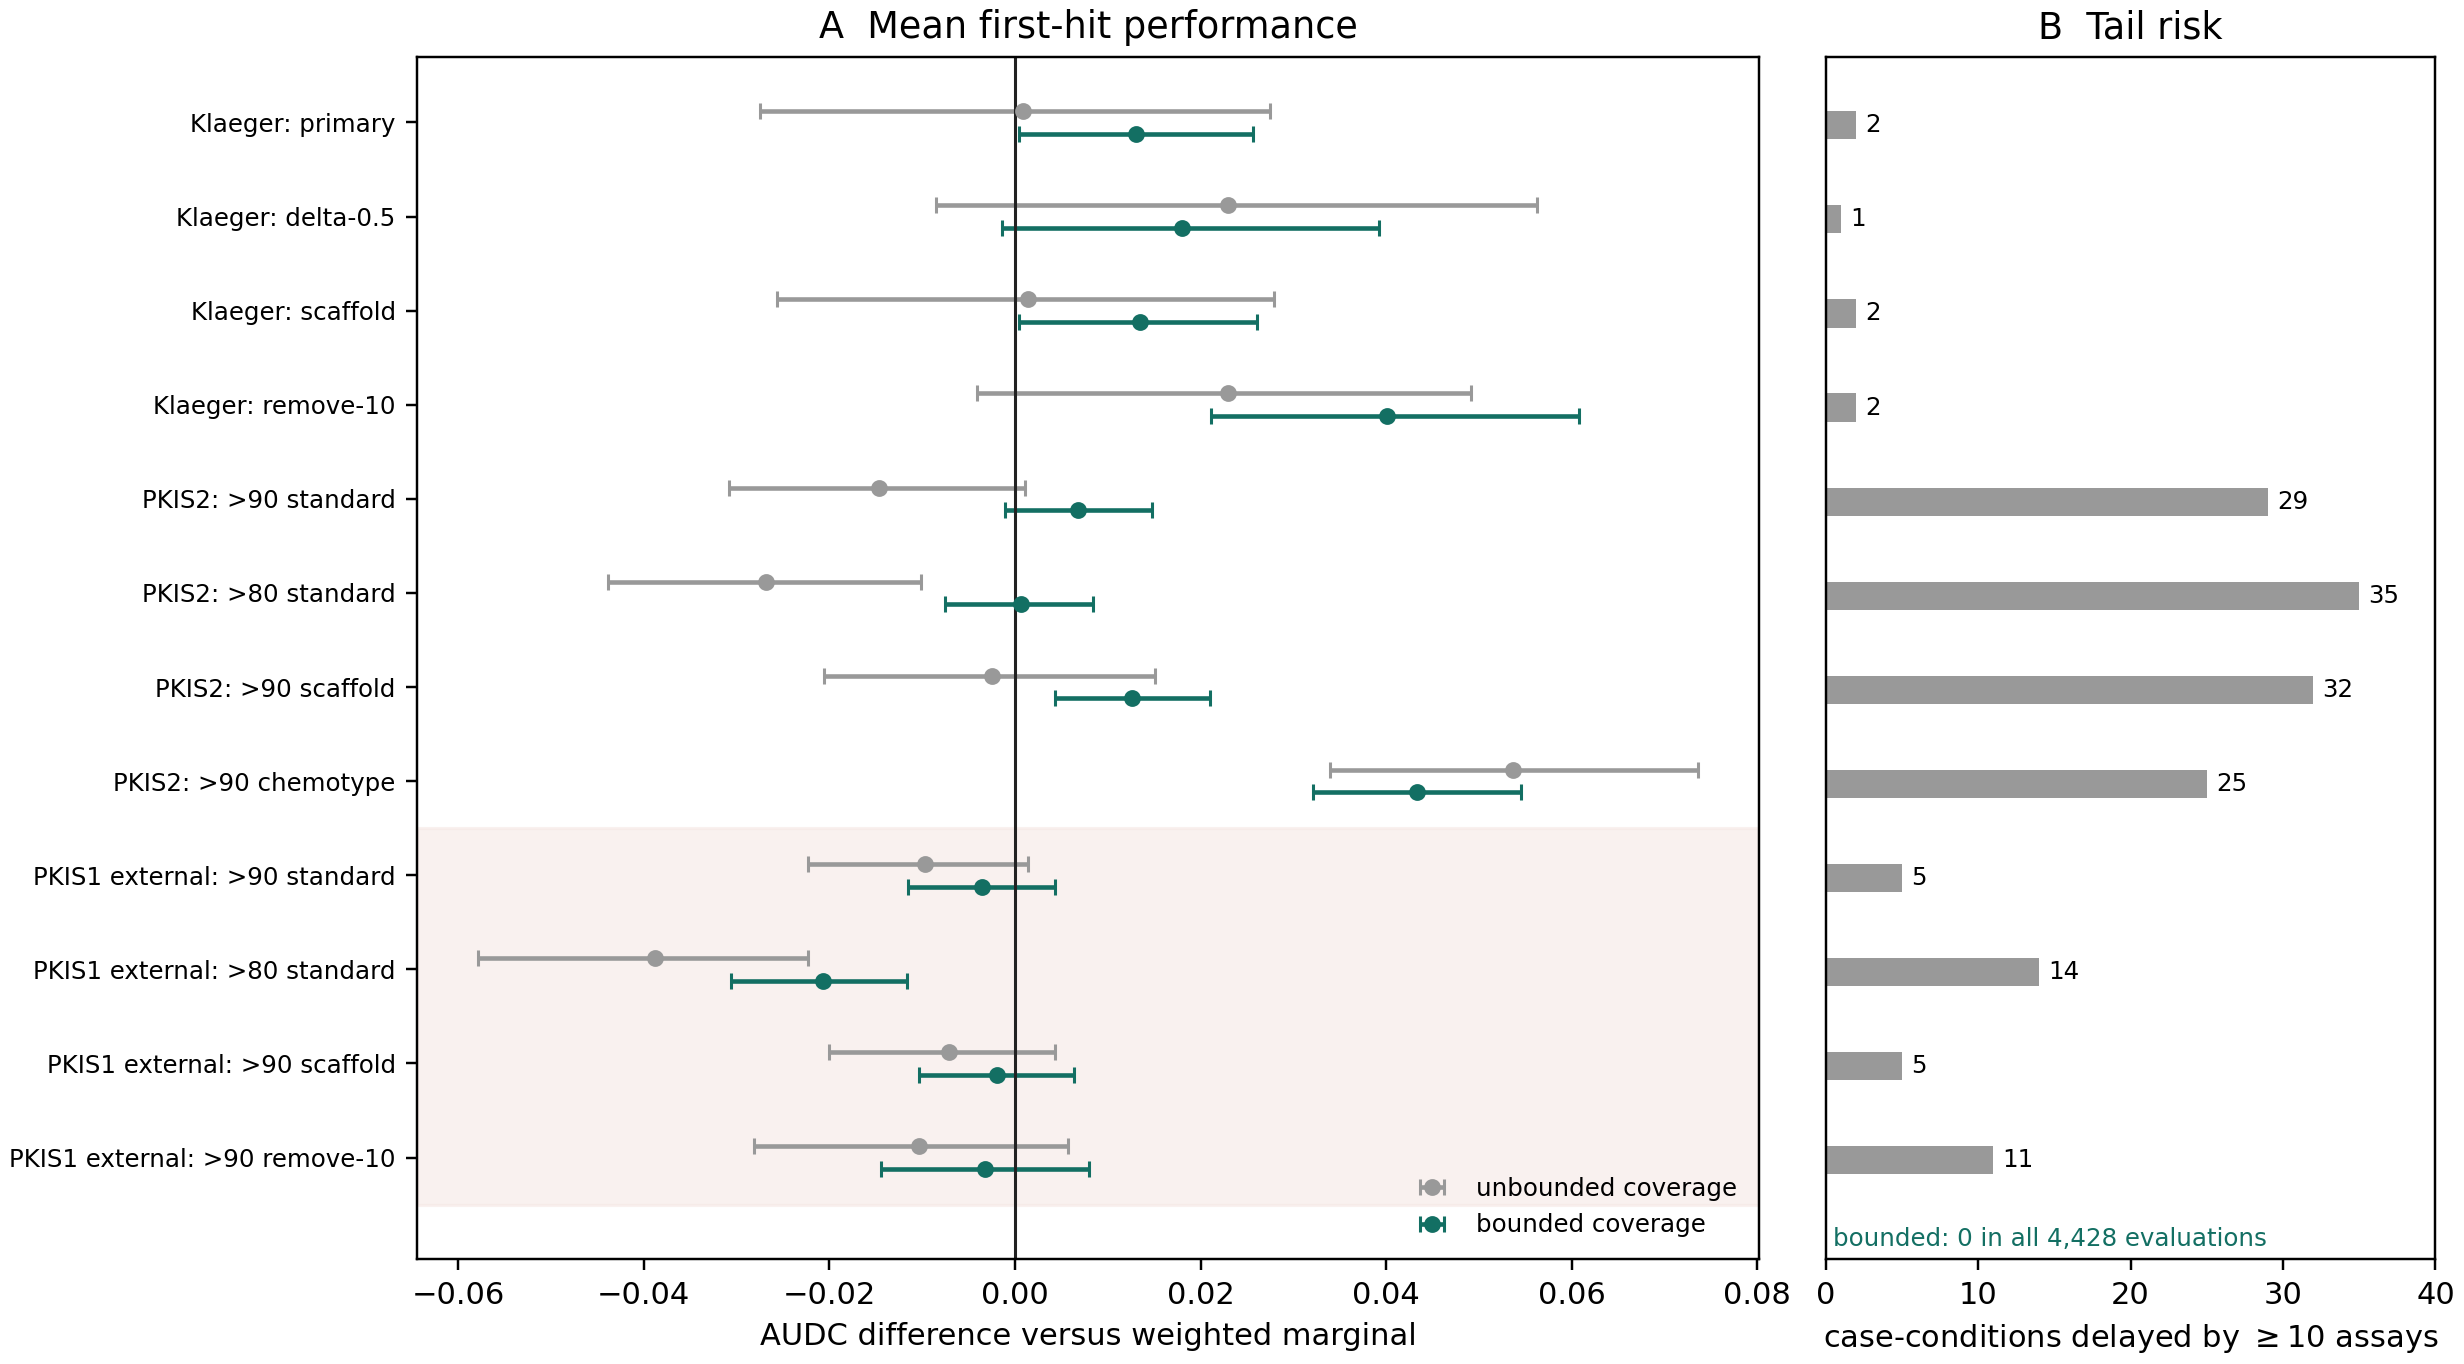
\includegraphics[width=\linewidth]{figures/bounded_cross_panel.png}
\caption{\textbf{A:} Paired mean AUDC effects with 95\% bootstrap intervals.
The shaded rows are the untouched PKIS1 external evaluation. \textbf{B:}
unconstrained coverage creates large first-hit delays; the rank-deadline rule
eliminates them by construction. Counts are compound--condition evaluations,
not independent compounds.}
\label{fig:main}
\end{figure}

\section{Results}

\paragraph{Development evidence favors bounded diversification.}
The bounded component was prespecified before its run, although promoting it
over a failed conformal wrapper occurred after results. Its effect versus
marginal ranking was nonnegative in all eight development conditions
(Fig.~\ref{fig:main}). Under PKIS2 chemotype exclusion, it gained 0.0433 AUDC
(95\% CI $[0.0321,0.0545]$), retaining 80.6\% of unbounded coverage's 0.0537
gain. PKIS2 scaffold exclusion gained 0.0127 ($[0.0043,0.0210]$). Klaeger
primary and remove-ten-nearest effects were 0.0131
($[0.00045,0.0257]$) and 0.0401 ($[0.0212,0.0608]$), respectively.

The bound repaired the main downside of unconstrained coverage. Unbounded
effects were negative for PKIS2 standard ($-0.0146$), $>80$ ($-0.0268$), and
scaffold ($-0.0025$), with 29, 35, and 32 large delays. Bounded effects were
$+0.0068$, $+0.0006$, and $+0.0127$, with zero large delays. Nevertheless,
bounded top-10 order stability under reference resampling was lower than
unbounded coverage by 0.0251 ($[-0.0303,-0.0198]$); stability is not claimed.

\begin{table}[t]
\caption{Untouched external PKIS1 effects. $\Delta$ is AUDC versus weighted
marginal. Delay is bounded minus marginal censored assays (positive is worse).
The frozen composite failed.}
\label{tab:external}
\centering
\small
\begin{tabular}{lrrrr}
\toprule
Condition & $\Delta$ bounded & 95\% CI & $\Delta$ unbounded & Mean delay\\
\midrule
$>90$ standard & $-.0035$ & $[-.0115,.0044]$ & $-.0097$ & $.070$\\
$>80$ standard & $-.0206$ & $[-.0306,-.0117]$ & $-.0388$ & $.413$\\
$>90$ scaffold & $-.0020$ & $[-.0104,.0063]$ & $-.0072$ & $.039$\\
$>90$ remove-10 & $-.0032$ & $[-.0145,.0080]$ & $-.0104$ & $.065$\\
\bottomrule
\end{tabular}
\end{table}

\paragraph{The external mean benefit does not transfer.}
All four PKIS1 bounded estimates were negative (Table~\ref{tab:external}); the
chemical-shift macro-effect was $-0.0026$ ($[-0.0113,0.0061]$). At $>80$ the
negative effect was decisive (sign-flip $p=10^{-5}$; four-condition Holm
$p=4\times10^{-5}$). Hence the external composite failed, and the data refute
a universal improvement claim.

The risk result did transfer. Bounded coverage had no delay of ten or more in
all 1,424 external evaluations; unbounded coverage had 35. Moreover, all four
bounded-versus-unbounded point estimates were positive: $+0.0062$ AUDC at $>90$ standard
($[0.0013,0.0124]$) and $+0.0181$ at $>80$
($[0.0096,0.0279]$). Reference-resampling stability was similar externally
($-0.0023$, $[-0.0097,0.0052]$).

\paragraph{The failure is not a parent-collapse artifact.}
An explicitly post-result 18-cell audit retained the negative verdict. At the
224 assay-construct resolution, standard effects remained negative at $>80$
($-0.0132$, $[-0.0222,-0.0049]$) and $>90$ ($-0.0090$,
$[-0.0187,0.0000]$). Parent-level standard effects were also negative at
thresholds $>50$, $>70$, $>80$, and $>90$. Two exploratory remove-ten cells
became positive at lower thresholds: $>50$ gained 0.0281
($[0.0111,0.0449]$, Holm over 18 $p=0.0141$) and $>70$ gained 0.0205
($[0.0059,0.0354]$, Holm $p=0.0968$). They define a possible regime
hypothesis; they do not rescue the frozen external test.

A separately frozen post-result PKIS2 audit kept all 406 assay constructs. Its
chemotype effect was 0.0442 ($[0.0336,0.0554]$; four-test Holm
$p=4\times10^{-5}$), essentially the parent-level 0.0433; its scaffold effect
was 0.0109 ($[0.0026,0.0193]$). Inclusive-boundary checks also retained the
chemotype conclusion at $\geq90$: 0.0353 at parent and 0.0367 at construct
resolution. Thus collapse does not create either aggregate headline, although
individual parent hits can remain construct-specific.

\section{Discussion}

The clean result is a separation between a guarantee and a prediction. Under
the weighted empirical-profile model, Eq.~\ref{eq:coverage} values diversity
because repeated assays on co-active profiles are redundant. That assumption
was useful for PKIS2 chemotype shift and Klaeger, but chemical similarity did
not make it transport to PKIS1. Rank deadlines cannot create transportability;
they ensure that being wrong about it has a controlled first-hit consequence.

This distinction is useful for resource-constrained drug discovery. If a team
has externally validated profile coverage for its assay platform and chemistry,
bounded coverage preserves much of the diversity gain without the observed
tail failures. Without such validation, marginal ranking remains the justified
default. A pseudo-outcome gate and a label-free conformal-support wrapper were
tested in the development sequence and did not solve this regime-selection
problem; we keep them as negative ablations rather than present a menu of
heuristics.

Important limitations remain. All evidence is retrospective. PKIS1 and PKIS2
are different compound panels but share the PKIS ecosystem; Klaeger adds a
different binding modality but only 111 compounds. Percent-inhibition
thresholds are operational labels, not potency estimates; their source paper
also calls threshold choice arbitrary. Max-collapsing assay constructs changes
the biological question, although construct-level audits did not reverse either
panel conclusion. Morgan similarity and reference profiles
omit target structure, concentration response, cell context, pharmacokinetics,
and assay cost. The method ranks kinase counter-screens; it neither predicts a
therapeutic window nor recommends a compound or treatment.

An AI-assisted source/data audit reviewed parent collapse, cross-platform
interpretation, label thresholds, all 35 large external delays, broad profiles,
and representative gains and losses. It found 11 PKIS1 and 13 PKIS2
multi-construct parent groups and released 288 underlying records for 63
flagged case-condition rows. This is not independent human expert sign-off or
biological validation; no such review is claimed. A named kinase-assay scientist
should still assess whether the any-construct and relative-affinity endpoints
match a real screening team's decision before prospective use.

\section{Conclusion}

Rank-deadline coverage gives an exact, inexpensive backstop for diversity-aware
kinase assay ordering. It preserved meaningful development gains and removed
all 163 large delays made by unconstrained coverage, but a frozen external
panel rejected universal mean improvement. For AI-enabled drug discovery, that
negative transfer is part of the contribution: a formal operational guarantee
can survive where a retrospective performance story does not.

\bibliographystyle{plainnat}
\bibliography{bounded_references}

\appendix
\section{Reproducibility and data rights}

The PKIS2 workbook is CC BY 4.0 and pinned by SHA-256
\texttt{48ead22a1...333e2a2c}. PKIS1 is a ChEMBL-derived raw export archived at
repository commit \texttt{5fd3934f...1294122b}, pinned by SHA-256
\texttt{81d7f9f8...119c88a9}, and redistributed only under ChEMBL's CC BY-SA
3.0 terms. The Klaeger-derived ChEMBL 30 records are also CC BY-SA 3.0. The
code records row-level provenance, versions, output hashes, and the chronology
of protocol, two input amendments, implementation freeze, external result, and
post-result robustness audit. Full runs are CPU-only, use no model training,
and incurred USD~0 in paid API use.

\section{Development-model sequence}

Unbounded profile coverage motivated the tail-risk criterion. A cross-fitted
pseudo-outcome gate removed the PKIS2 $>80$ reversal and reduced chemotype
large delays from 25 to 10, but retained only 57.4\% of the chemotype gain and
reduced stability. A label-free conformal-support gate retained 78.3\% and
reduced the delay count to 21, missing the fixed limit by one and again reducing
stability. The final conformal wrapper around bounded coverage retained 60.1\%
and failed its composite. The prespecified bounded component passed five of six
development criteria; selecting it as the headline after observing that run is
why PKIS1 was required.

\section{Biological-review handoff}

The release includes the completed computational/literature review, full
construct mappings, threshold-boundary audit, all flagged cases, and source
records. Independent human attestation remains explicitly outstanding. Any
later revision following expert feedback must distinguish interpretation
corrections from outcome-driven changes to the algorithm. A
future decisive experiment is a preregistered prospective or time-split kinase
panel in a discovery-relevant chemical series, with assay costs and confirmation
measurements specified before ranking.

\end{document}
